%\section{Appendix}
\section{Sampling Accumulation Curves}

\begin{center}
	\begin{figure}[H]
		\subfloat[Species per locality]{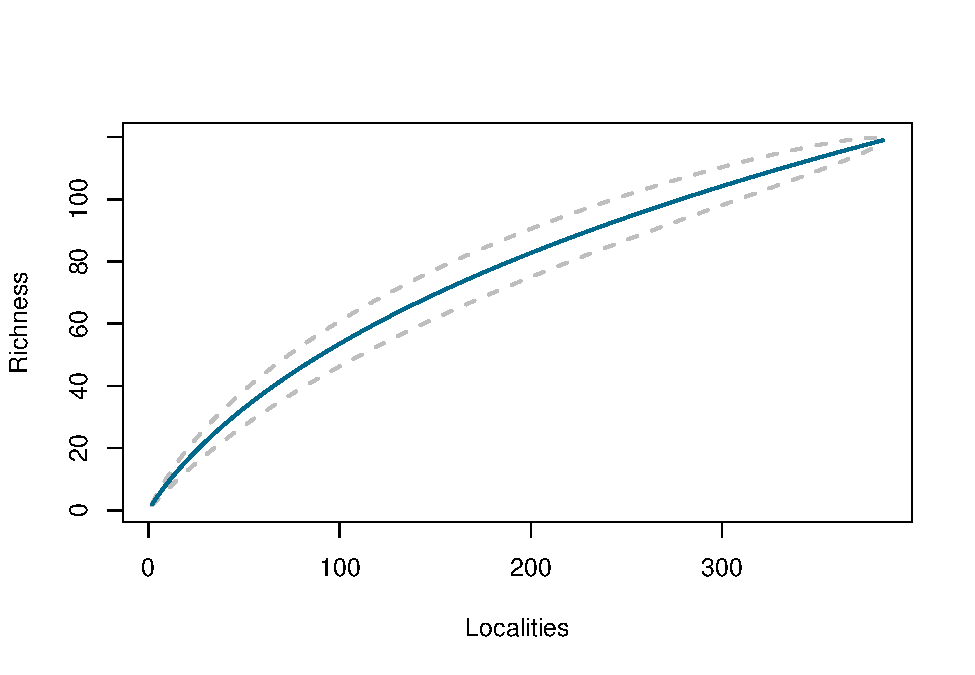
\includegraphics[scale=0.3]{MA_JJ_files/figure-latex/SACSpecies-1.pdf}}
		\subfloat[Species per reference]{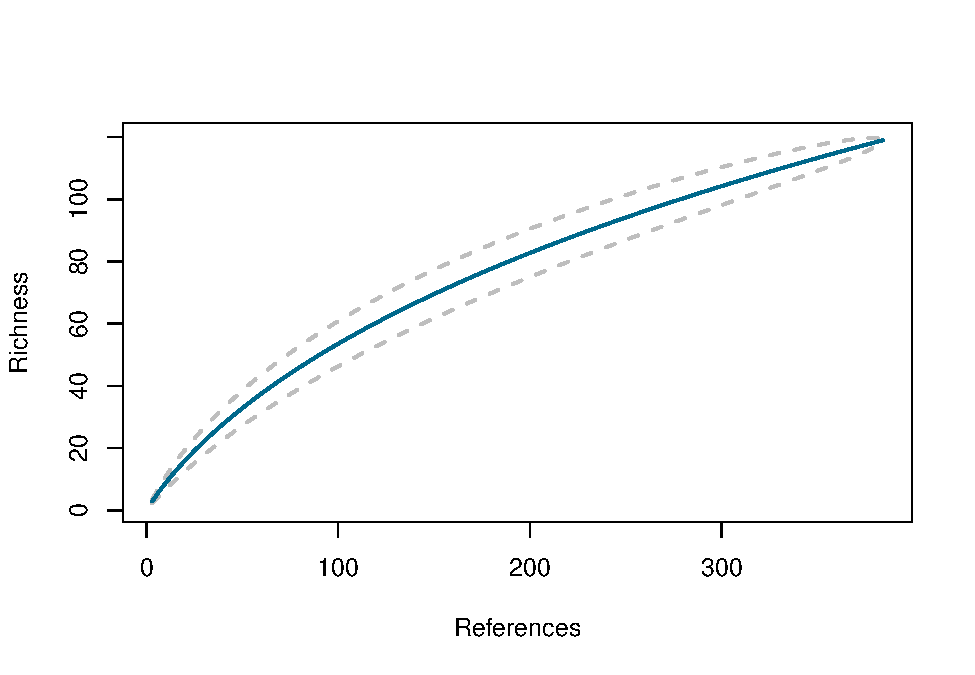
\includegraphics[scale=0.3]{MA_JJ_files/figure-latex/SACSpecies-2.pdf}}	\subfloat[Africa]{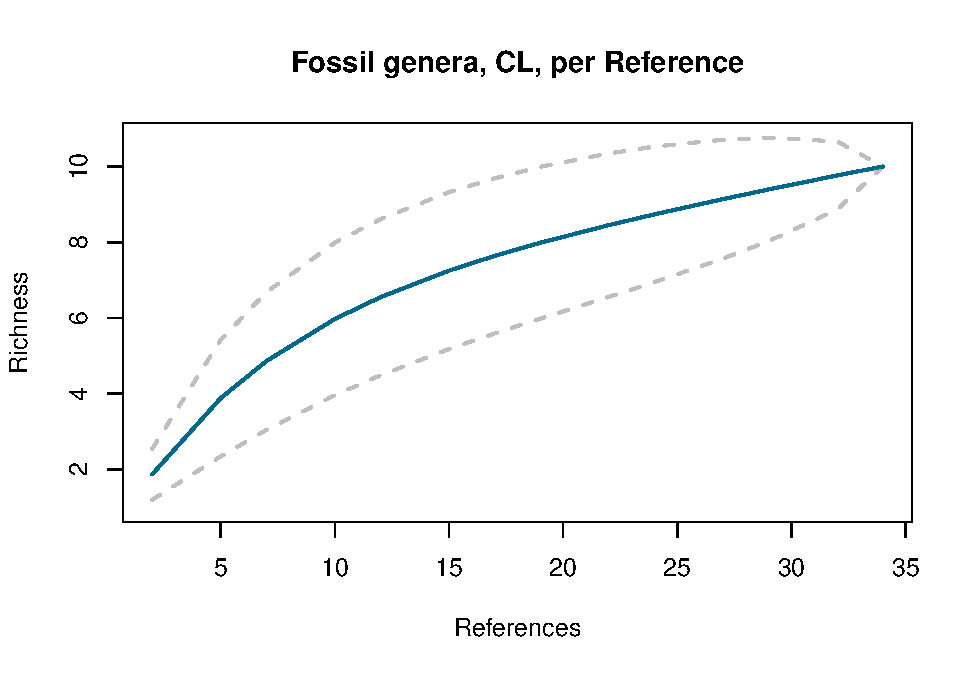
\includegraphics[scale=0.3]{MA_JJ_files/figure-latex/SACGAfrica-1.pdf}}
		\hfill %
		\subfloat[America]{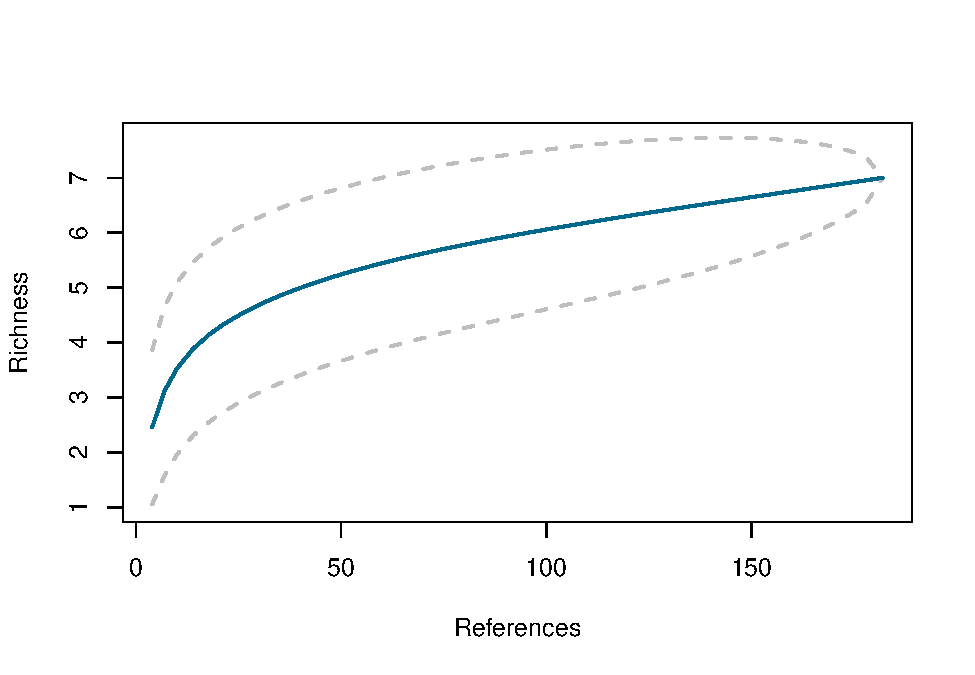
\includegraphics[scale=0.3]{MA_JJ_files/figure-latex/SACGAmerica-1.pdf}}
		\subfloat[North America]{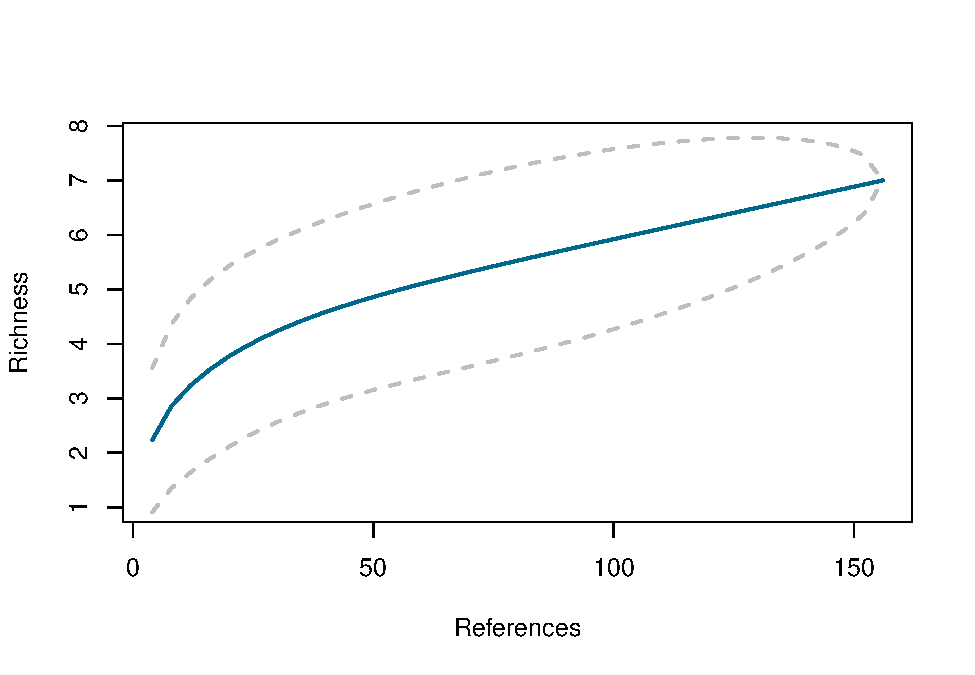
\includegraphics[scale=0.3]{MA_JJ_files/figure-latex/SACGNAmerica-1.pdf}}
		\subfloat[South America]{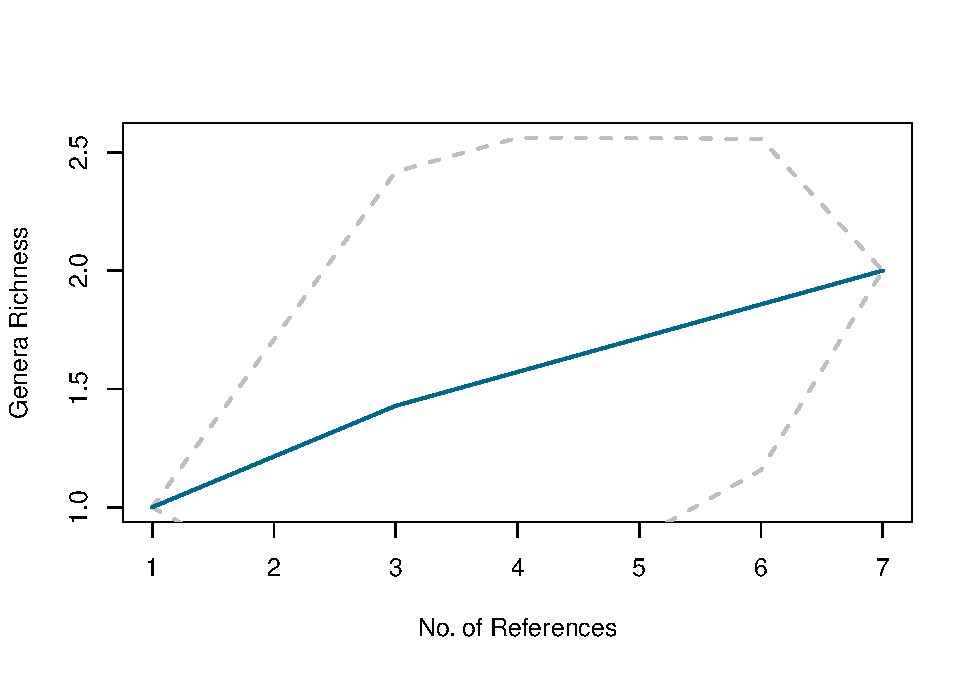
\includegraphics[scale=0.3]{MA_JJ_files/figure-latex/SACGSAmerica-1.pdf}}
		\hfill %
		\subfloat[Asia]{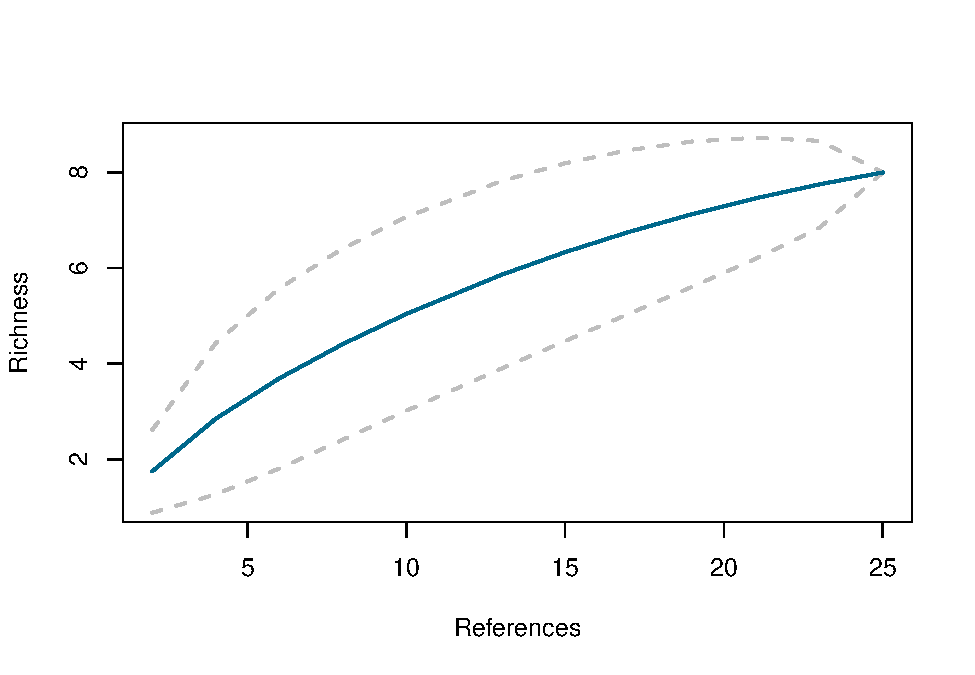
\includegraphics[scale=0.3]{MA_JJ_files/figure-latex/SACGAsia-1.pdf}}
		\subfloat[Europe]{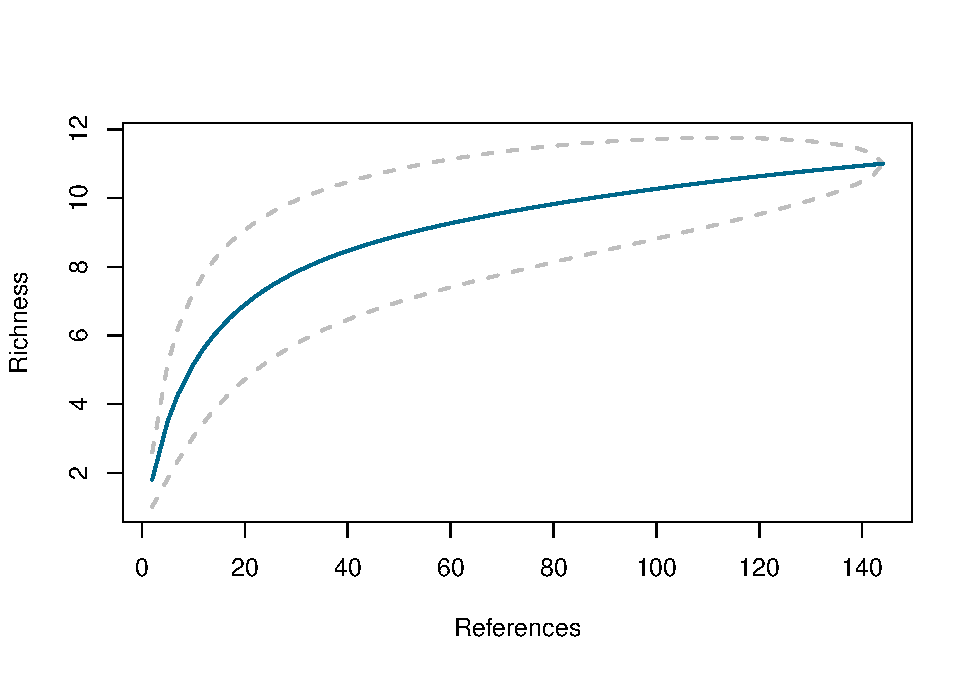
\includegraphics[scale=0.3]{MA_JJ_files/figure-latex/SACGEurope-1.pdf}}
		\subfloat[Eurasia]{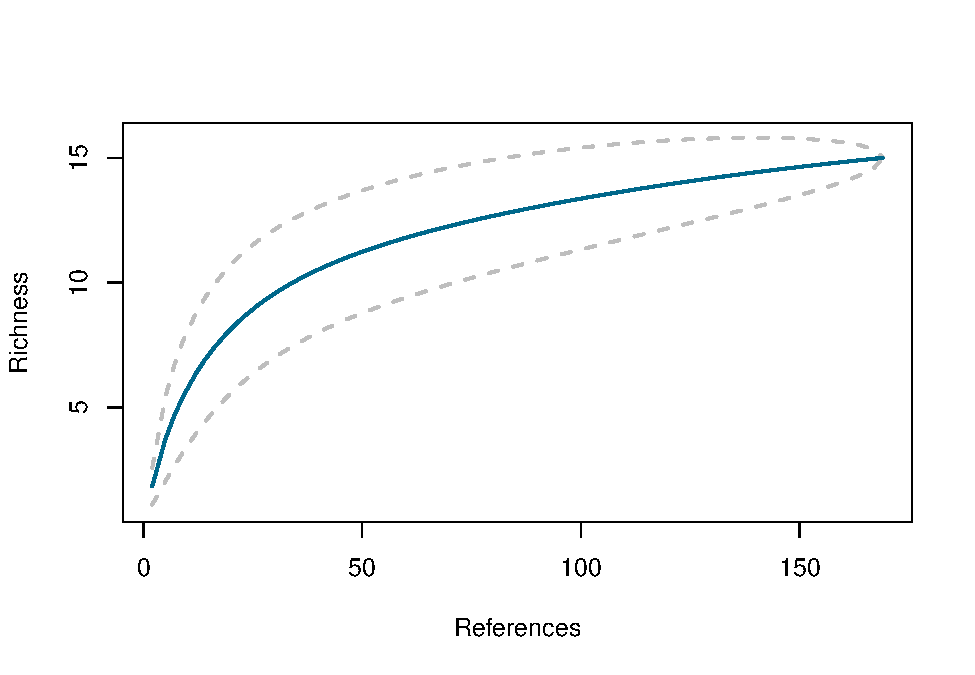
\includegraphics[scale=0.3]{MA_JJ_files/figure-latex/SACGEurasia-1.pdf}}
		\caption[Additional Sampling Accumulation Curves]{Sampling Accumulation Curves: (a) - (b) Species are not sufficiently sampled, regardless of sampling unit. (c) - (i) Sampling Accumulation Curves on generic level per continent. Only Europe (h) and Eurasia (i) are sufficiently sampled.}
		\label{fig:SACall}
	\end{figure}
\end{center}

\FloatBarrier
